\documentclass[a4paper]{article}
\usepackage[italian]{babel}
\usepackage{hyperref}
\usepackage{tipa}
\usepackage{graphicx}
\usepackage{minted}

\author{Diego Roberto Ammirabile 0001021216 \\ \texttt{diego.ammirabile@studio.unibo.it}}
\date{Febbraio 2025}
\title{Report}
\begin{document}
\maketitle
\tableofcontents
\paragraph{Panoramica del progetto}
\subparagraph{Obiettivi}

\paragraph{Dettagli di implementazione}
Il progetto è stato realizzato attraverso grazie al framework \texttt{Ionic} combinato con il framework \texttt{Vue}. Quando possibile è stato utilizzato il \texttt{Capacitor} per accedere alle funzionalità native dei dispositivi mobili, questo non è sempre stato possibile a causa di limitazioni del framework. Per avere una migliore gestione dei tipi è stato utilizzato \texttt{TypeScript}. Il progetto è stato inizializzato con \texttt{Vite}.

\subparagraph{Struttura del codice}
Il codice è stato organizzato in componenti Vue, in modo da rendere il codice più modulare e manutenibile. Ogni componente è stato progettato per essere il più possibile indipendente dagli altri, in modo da poter essere riutilizzato in altri contesti. Esistono tuttavia componenti che non trovano applicazione in altri contesti se non quello del sovra-componente, tali componenti però gestiscono parti di logica differente da quella del sovra-componente, per cui è stato ritenuto utile mantenerli separati.
Il filesystem ha quindi la seguente struttura:
\begin{itemize}
	\item \texttt{android/} contiene i file necessari per la compilazione dell'applicazione per Android
	\item \texttt{dist/} contiene i file compilati
	\item \texttt{node\_modules/} contiene le dipendenze del progetto
	\item \texttt{public/} contiene i file statici
	\item \texttt{src/} contiene il codice sorgente
		\begin{itemize}
			\item \texttt{components/} contiene i componenti Vue
			\item \texttt{router/} contiene il router
			\item \texttt{theme/} contiene i file di stile
			\item \texttt{utils/} contiene le utility
			\item \texttt{views/} contiene le viste
			\item \texttt{App.vue} è il file principale
			\item \texttt{interfaces.ts} contiene le interfacce
			\item \texttt{main.ts} è il file principale
			\item \texttt{variables.json} contiene le variabili, di fatto solo l'URL dell'API
			\item \texttt{vite-env.d.ts} contiene le variabili di ambiente
		\end{itemize}
	\item \texttt{capacitor.config.ts} contiene la configurazione di Capacitor
	\item \texttt{cypress.config.ts} contiene la configurazione di Cypress
	\item \texttt{index.html} è il file principale
	\item \texttt{ionic.config.json} contiene la configurazione di Ionic
	\item \texttt{LICENSE} contiene la licenza
	\item \texttt{package-lock.json} contiene le dipendenze con le versioni esatte
	\item \texttt{package.json} contiene le dipendenze
	\item \texttt{ProjectsLAM2024.pdf} contiene il progettato
	\item \texttt{README.md} contiene le informazioni sul progettato
	\item \texttt{tsconfig.json} contiene la configurazione di TypeScript
	\item \texttt{tsconfig.node.json} contiene la configurazione di TypeScript per Node
	\item \texttt{vite.config.ts} contiene la configurazione di Vite
\end{itemize}

\paragraph{Interfaccia utente}


% login.png
% signup.png
% record.png
% recorded-audio.png
% redorded-uploaded.png
% map-pins.png
% map-audio-info.png
% map-audio-submenu.png
% saved.png
% saved-infos.png

La prima schermata che si presenta all'utente è quella di login,
\begin{figure}[h]
	\centering
	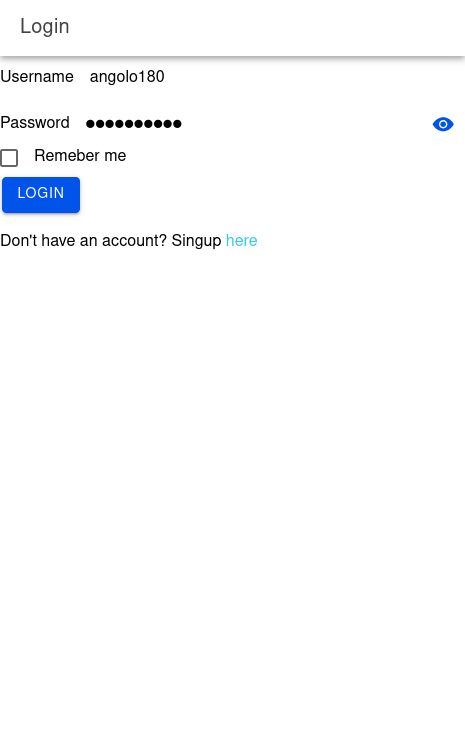
\includegraphics[width=0.5\textwidth]{login.png}
	\caption{Schermata di login}
\end{figure}

\begin{figure}[h]
	\centering
	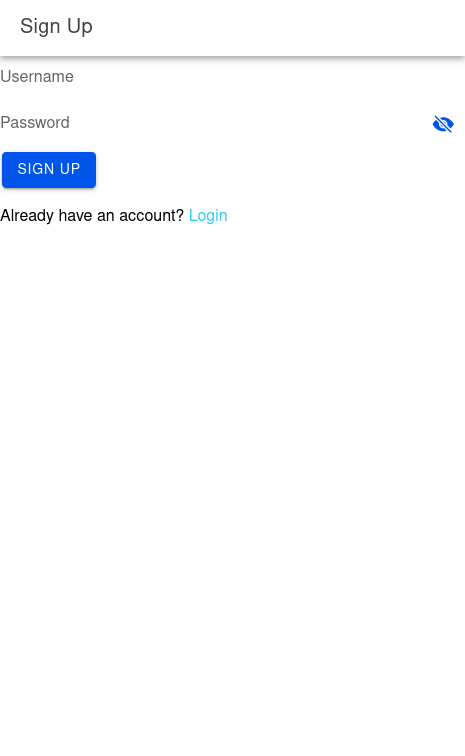
\includegraphics[width=0.5\textwidth]{signup.png}
	\caption{Schermata di registrazione}
\end{figure}

\begin{figure}[h]
	\centering
	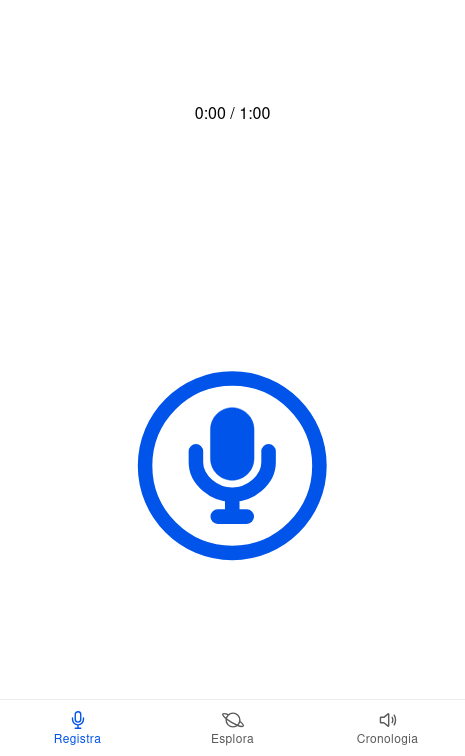
\includegraphics[width=0.5\textwidth]{./record.png}
	\caption{Schermata di registrazione audio}
\end{figure}

\begin{figure}[h]
	\centering
	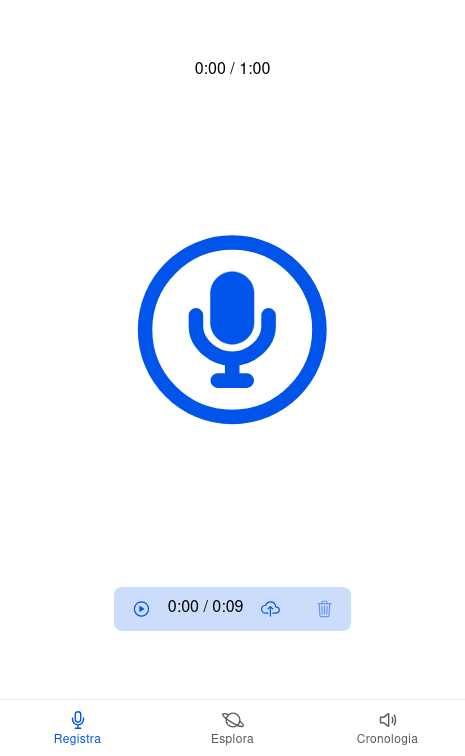
\includegraphics[width=0.5\textwidth]{./recorded-audio.png}
	\caption{Schermata di registrazione audio con audio registrato}
\end{figure}

\begin{figure}[h]
	\centering
	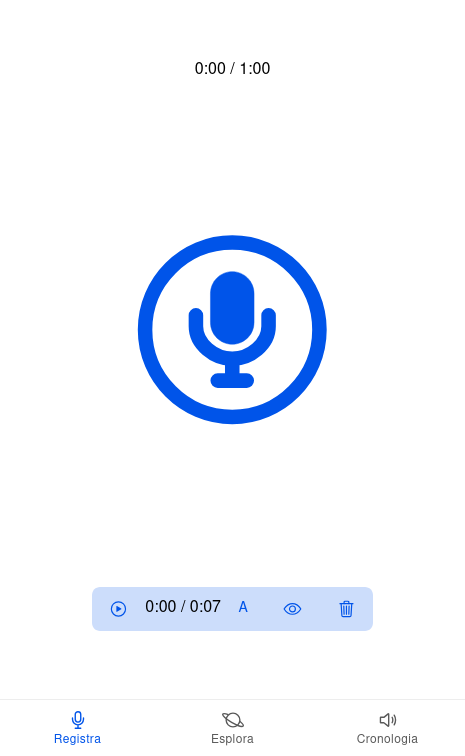
\includegraphics[width=0.5\textwidth]{./redorded-uploaded.png}
	\caption{Schermata di registrazione audio con audio caricato}
\end{figure}

\begin{figure}[h]
	\centering
	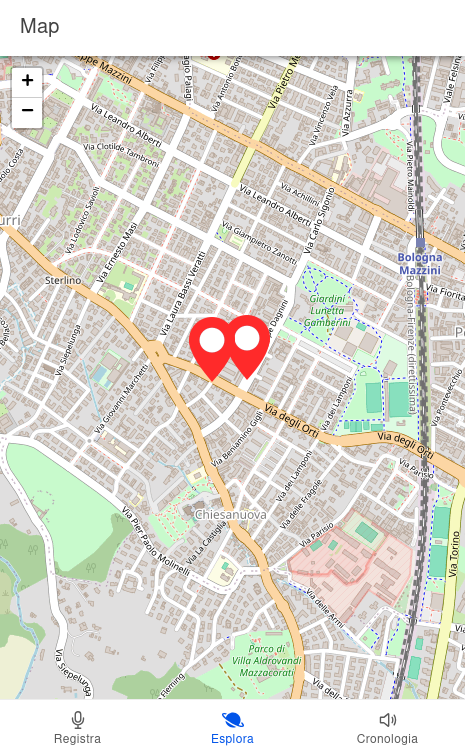
\includegraphics[width=0.5\textwidth]{./map-pins.png}
	\caption{Schermata della mappa con i pin}
	
\end{figure}

\begin{figure}[h]
	\centering
	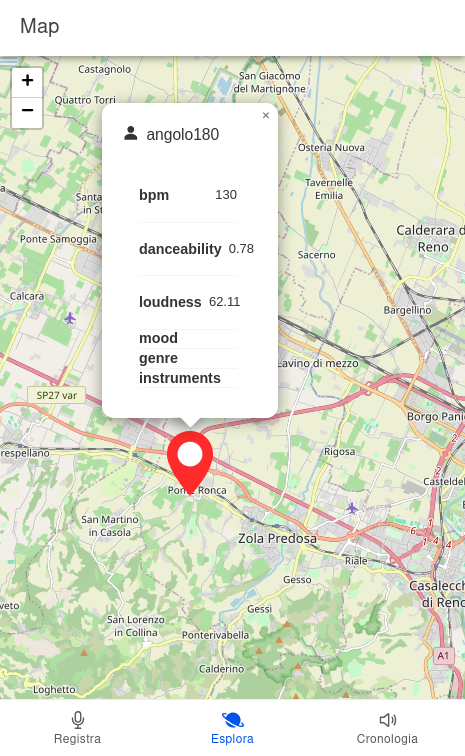
\includegraphics[width=0.5\textwidth]{./map-audio-info.png}
	\caption{Schermata della mappa con le informazioni dell'audio}
\end{figure}

\begin{figure}[h]
	\centering
	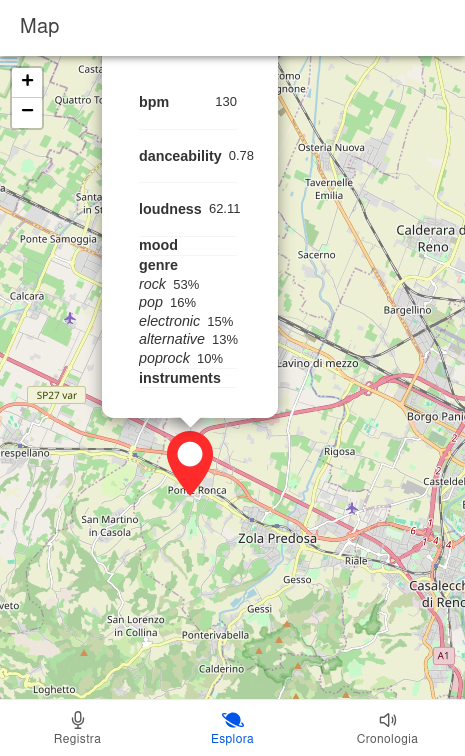
\includegraphics[width=0.5\textwidth]{./map-audio-submenu.png}
	\caption{Schermata della mappa con il submenu dell'audio}
\end{figure}

\begin{figure}[h]
	\centering
	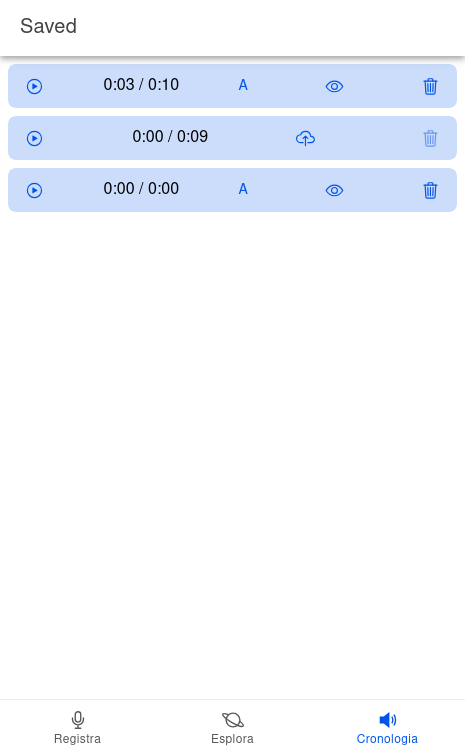
\includegraphics[width=0.5\textwidth]{./saved.png}
	\caption{Schermata dei salvati}
\end{figure}

\begin{figure}[h]
	\centering
	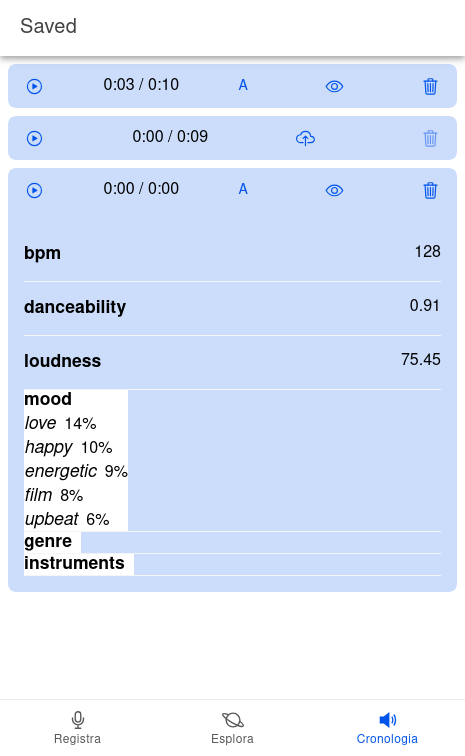
\includegraphics[width=0.5\textwidth]{./saved-infos.png}
	\caption{Schermata dei salvati con le informazioni}
\end{figure}



\begin{minted}{typescript}
export interface User {
	id: number;
	name: string;
	email: string;
	phone: string;
}
\end{minted}

\paragraph{Conclusioni}
\end{document}
